%!TEX root = Report.tex
\chapter{Versuchsaufbau}\label{sec:experimentalsetup}

In Abbildung \ref{pic:versuchsaufbau} ist die Versuchsanordung zu sehen. Stickstoff strömt in einen Rohrofen und wird erwärmt. Die Gastemperatur soll nun mit einem Thermolement, welches die Temperatur misst, ermittelt werden. Wie es oben erwähnt wurde, die Messung wird erheblich durch die Wärmestrahlung beeinflusst, deswegen schirmt man das Thermolement ab (Abbildung \ref{pic:lanze}). Zusätzlich wird eine bekannte Konvektion erzwungen. Dies reduziert die Temperatur des Thermoelements und kühlt es fast auf die Gastemperatur.\\

\begin{figure}[H]
\centering
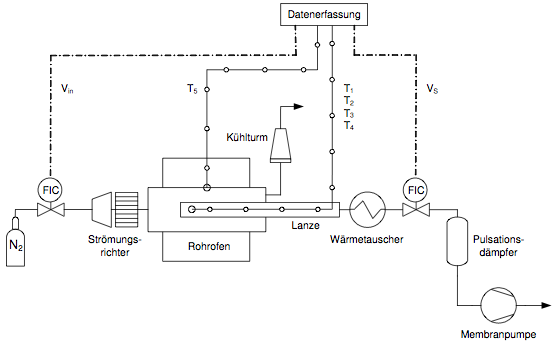
\includegraphics[width=\textwidth]{pics/versuchsaufbau.png}
\caption{Schematische Versuchsanordnung}
\label{pic:versuchsaufbau}
\end{figure}

Der in den Ofen eintretende Gasstrom kann mittels Massendurchflussmesser gemessen und geregelt werden. Eine Lanze/Absaugvorrichtung saugt mithilfe einer Membranpumpe einen Teil des Gases ab. Der Aufbau der Lanze ist in Abbildung \ref{pic:lanze} zu sehen. Insgesamt werden durch vier Thermoelemente vier Temperaturen gemessen. $T_1$ ist die verfälschte Gastemperatur, $T_2$ die Temperatur am geschützten Thermoelement und $T_3$ und $T_4$ die Temperaur des Schirms (für die Berechnung wird die Schirmtemperatur gemittelt). Die Datenerfassung der gemessenen Temperaturen übernimmt ein Computer. Das abgesaugte Gas wird danach gekühlt, um die nachfolgenden Instrumente nicht allzu hohen Temperaturen auszusetzen. Der folgende Massendurchflussregler regelt und bestimmt den Gasstrom. Anschliessend geht das Gas an die Umgebung. Der grösste Teil des Gases wird jedoch nicht abgesaugt, sondern verlässt den Ofen und wird in einem Kühlturm auf Umgebungstemperatur gebracht und verlässt dann den Ofen. \\

\begin{figure}[H]
\centering
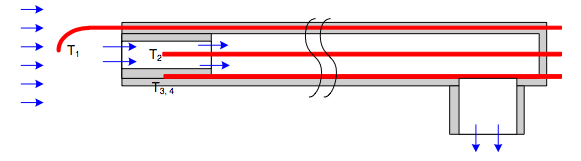
\includegraphics[width=\textwidth]{pics/lanze.png}
\caption{Querschnitt Absaugvorrichting/Lanze mit den Thermoelementen (rot)}
\label{pic:lanze}
\end{figure}

In unserem Experiment werden die Temperaturen $T_1$, $T_2$, $T_3$ und $T_4$ bei zwei verschiedenen Ofentemperaturen $T_H$ und jeweils drei unterschiedlichen Absaugvolumenströmen $V_s$ gemessen.

